\begin{enumerate}[label=\thesection.\arabic*.,ref=\thesection.\theenumi]
\numberwithin{equation}{enumi}
\item A unity negative feedback system has the open loop transfer function \\
\begin{align}
    G(s) = \frac{K}{s(s+1)(s+3)} 
    \label{eq:t1}
\end{align}
The value of the gain K ($>$0) at which the root locus crosses the imaginary axis is ?

\solution

\item Root Locus: \\
	  The Root locus is the locus of the roots of the characteristic equation, which are the poles of closed loop transfer function, by varying system gain K from $0$ to $\infty$.

\item The characteristic equation of the closed loop control system is: 

    \begin{align}
         1 + G(s)H(s) = 0    
    \end{align}
    
    The points on the root locus branches must satisfy the \textbf{angle condition.}
    We can find the value of K for the points on the root locus branches by using \textbf{magnitude condition.}

\item Angle Condition: \\
    Given the Characteristic equation, we can write it as:
    \begin{align}
         G(s)H(s) = -1 + j0   
    \end{align}
    The phase angle of G(s)H(s) is:
    $\angle$G(s)H(s) =\[ \arctan(\frac{0}{-1}) = (2n+1)\pi\]
    The angle condition is the point at which the angle of the transfer function is an odd multiple of 180.
   
\item Magnitude Condition \\

    Magnitude of G(s)H(s) is:
    \begin{align}
        |G(s)H(s)| = \sqrt{(-1)^2 + 0^2}
    \end{align}
    $\implies$
    \begin{align}
        |G(s)H(s)| =1 
    \end{align}
    The magnitude condition is that the point (which satisfied the angle condition) at which the magnitude of the transfer function is one.

\item For given transfer function: \\
    H(s) = 1. So, closed loop transfer function will be
    \begin{align}
        T(s) = \frac{K}{s(s+1)(s+3)+K}
    \end{align}
    Poles of closed loop transfer function are the roots of the Characteristic Equation.
    So, characteristic Equation is:
    \begin{align}
        s^3 + 4s^2 + 3s + K = 0
    \end{align}

\item Routh Array Table:\\
    \textbf{If all elements of any row of the Routh array table are zero, then the root locus branch intersects the imaginary axis}\\
    Routh Array Table:
    \begin{align}
        \mydet{s^3\\s^2\\s^1\\s^0}
        \mydet{1 & 3\\ 4 & K \\ (12-K)/4 & 0 \\ K}
    \end{align}\\
    For poles to be on imaginary axis, row $s^1$ should be zero. So,     
    \begin{align}
        \frac{12-K}{4} = 0
    \end{align}\\
    Hence, K = 12.

\item Verification: \\
    Auxilliary equation:
    \begin{align}
        4s^2 + K = 0
    \end{align}
    \begin{align}
        4s^2 + 12 = 0
    \end{align}
    $\implies$s = $-j\sqrt{3}$,$+j\sqrt{3}$\\ 
    Thus a pair of poles lie on imaginary axis for K = 12.
   

\item Root Locus plot

	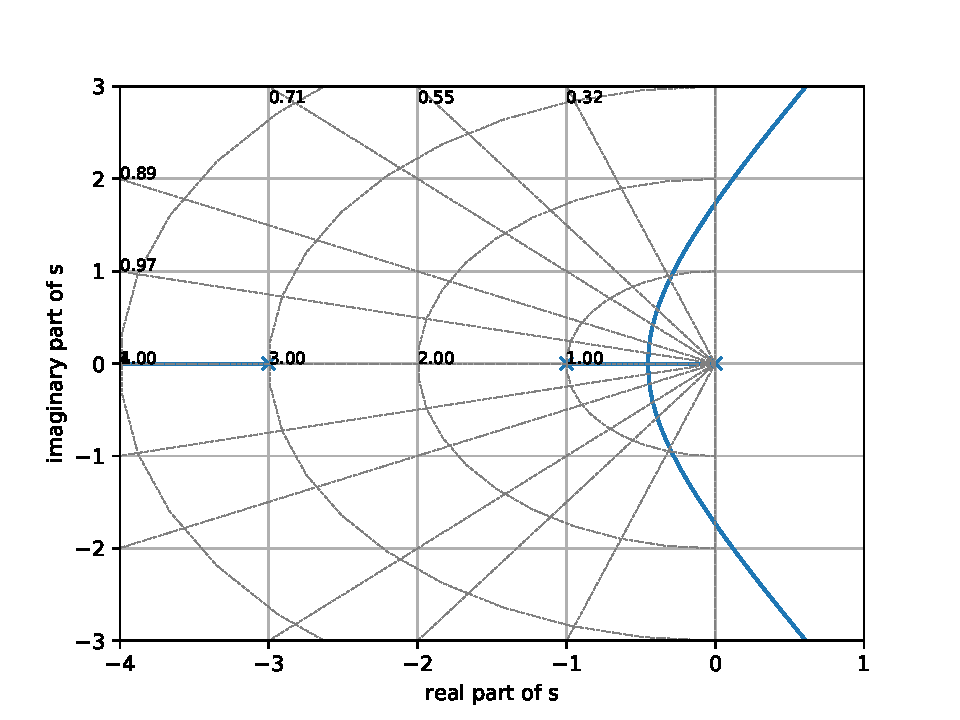
\includegraphics[width=\columnwidth]{./figs/ee18btech11050.pdf}
Code to plot root locus:
\begin{lstlisting}
codes/ee18btech11050.py
\end{lstlisting}    

\end{enumerate}
